\documentclass{config/apuntes}

\title{Redes Biológicas y Biología de Sistemas}
\author{Sandra Mingo Ramírez}
\date{2024/25}
\acronym{RBBS}

\usepackage[all]{nowidow}
\usepackage{listing}
\usepackage{color}
\usepackage{tabularx}
\usepackage{multirow}
\usepackage{makecell}
\usepackage{amsmath}
\usepackage{array}
\usepackage{mathtools}
\usepackage{soul}

\definecolor{dkgreen}{rgb}{0,0.6,0}
\definecolor{gray}{rgb}{0.5,0.5,0.5}
\definecolor{mauve}{rgb}{0.58,0,0.82}

\lstset{
  frame=tb,
  aboveskip=3mm,
  belowskip=3mm,
  showstringspaces=false,
  columns=flexible,
  basicstyle={\small\ttfamily},
  numbers=none,
  numberstyle=\tiny\color{gray},
  keywordstyle=\color{blue},
  commentstyle=\color{dkgreen},
  stringstyle=\color{mauve},
  breaklines=true,
  breakatwhitespace=true,
  tabsize=3
}

\usepackage{tocloft}

\advance\cftchapnumwidth 0.9em\relax
\advance\cftsecnumwidth 0.6em\relax
\advance\cftsubsecindent 0.5em\relax
\advance\cftsubsecnumwidth 0.5em\relax
\begin{document}

\begin{abstract}
La biología de sistemas busca entender la importancia de cuantificar en biología y poder formular algunos problemas biológicos en modelos matemáticos relativamente simples. Los modelos son siempre simplificaciones grandes de los sistemas biológicos complejos. Muchas veces, esas simplificaciones no son abstractas, si no que reflejan el conocimiento que se tiene de los sistemas. No obstante, todos son imperfectos, ya que no contienen toda la información posible. Como decía el estadístico George Box, todos los modelos son erróneos, pero algunos son útiles. Por eso, en esta asignatura aprenderemos a cuantificar en biología y construir modelos matemáticos.
\end{abstract}

\pagestyle{plain}

\maketitle

\tableofcontents

%GUÍA DOCENTE
%Ejercicios 60%
%Memoria 15%
%Defensa 15%
%Participación 10%

%50% Teoría: 40% examen preguntas cortas/problemas, 60% projecto en grupo
%50% Prácticas: 

%30/01 - Raúl Guantes
\chapter{Conceptos básicos}
\section{La importancia de cuantificar y estimar las escalas en biología}
La biología de sistemas es un campo que busca entender los sistemas biológicos a través de la cuantificación y la modelización matemática. Los modelos matemáticos son simplificaciones de sistemas biológicos complejos, y aunque no son perfectos (ya que no pueden capturar toda la información), son útiles para entender y predecir comportamientos biológicos. Como dijo el estadístico George Box: "Todos los modelos son erróneos, pero algunos son útiles".

Una herramienta clave en este campo es BioNumbers, una base de datos que recopila información cuantitativa en biología. Esta información es esencial para interpretar resultados experimentales y diseñar nuevos experimentos. Por ejemplo, al realizar experimentos, es fundamental calcular la media y la desviación estándar de los resultados para estimar el error. El error se redondea a una cifra significativa, y la medida se expresa con la misma precisión que el error.

\subsection{Estimación de la expresión de proteínas en \textit{E. coli}}
Supongamos que encontramos una proteína en un cultivo celular de \textit{E. coli} con una concentración de 1 picoMolar (pM) por célula. ¿Es esta expresión significativa? Para responder, necesitamos calcular el número de moléculas de la proteína por célula, lo que depende del volumen celular.

\paragraph{Datos} Las bacterias tienen forma cilíndrica con una longitud de 2 micras y un diámetro de 1 micra. La concentración de la proteína: $C = 1 pM = 10^{-12}M$.

\paragraph{Cálculos}
\begin{enumerate}
\item Volumen de la célula
$$V = \pi r^2 h \rightarrow \pi (0,5 \mu m)^2 2 \approx 1,5 \mu m^3 = 1,5 \cdot 10^{-15} l = 1,5 fl$$
\item Número de moléculas de proteína por célula
$$C = \frac{N_p}{V \cdot N_{av}} \rightarrow N_p = C \cdot V \cdot N_{av}$$
$$N_p = C \cdot V \cdot N_{av} = 10^{-12}M \cdot 1,5 \cdot 10^{-15}l \cdot 6 \cdot 10^{23} \approx 10^{-3} molecules$$
Esto significa que hay aproximadamente 1 molécula de proteína por cada 1.000 células.
\end{enumerate}

De esta forma, podemos decir que como regla general, una concentración de 1 nanomolar (nM) en \textit{E. coli} corresponde aproximadamente a 1 molécula por célula, dado que el volumen de una célula de \textit{E. coli} es del orden de 1 fl.

\subsection{Variabilidad en la cuantificación de proteínas}
En \textit{E. coli}, la cantidad de proteínas se ha cuantificado utilizando dos técnicas principales: espectrometría de masas y microscopía de fluorescencia. Estas técnicas arrojan resultados diferentes:
\begin{itemize}
\item En espectrometría de masas, el número promedio de una proteína cualquiera en \textit{E. coli} es de 1.000-2.000 moléculas.
\item En microscopía de fluorescencia, este número es de alrededor de 50 moléculas.
\end{itemize}

\begin{figure}[h]
\centering
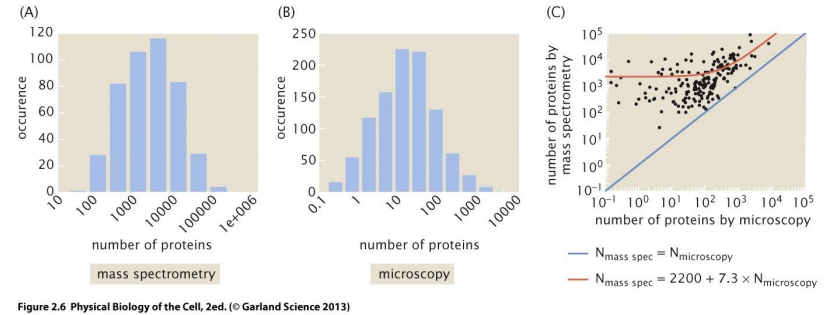
\includegraphics[width = 0.9\textwidth]{figs/mol-census.png}
\end{figure}

Para \textbf{proteínas muy abundantes}, ambas técnicas muestran una buena correlación.
Para \textbf{proteínas poco abundantes}, la correlación se pierde debido a la variabilidad intrínseca en la expresión génica. Esto no es un artefacto experimental, sino una consecuencia de la estocasticidad en los procesos biológicos (limitación física). Cuando el número de copias de una proteína es bajo, la probabilidad de que ocurran reacciones bioquímicas al azar es menor. Esto genera una gran variabilidad en la cantidad de proteínas entre células genéticamente idénticas. En cambio, cuando el número de copias es alto, las reacciones ocurren con mayor frecuencia, reduciendo la variabilidad.

\subsection{Consecuencias numéricas en biología}
La expresión génica es un proceso altamente estocástico debido al bajo número de copias de muchas moléculas involucradas (ADN, factores de transcripción, ARN polimerasa, etc.). Esto tiene varias implicaciones:
\begin{itemize}
\item \textbf{Variabilidad celular:} Incluso en poblaciones de células clonales en el mismo ambiente, la expresión de proteínas varía significativamente. Por ejemplo, las huellas dactilares de dos gemelos son diferentes debido a esta variabilidad.
\item \textbf{Estocasticidad como mecanismo evolutivo:} La aleatoriedad en la expresión génica puede ser aprovechada para generar diversidad. Por ejemplo, en \textit{Bacillus subtilis}, algunas células entran en estado de esporulación en ausencia de nutrientes, mientras que otras continúan dividiéndose.
\end{itemize}

\subsection{Ejemplo: distancia media entre proteínas en una célula de \textit{E. coli}}
La distancia entre proteínas en una célula es inversamente proporcional a la concentración de proteínas (a mayor concentración de proteínas, menos distancia entre ellas). Matemáticamente, siendo c la concentración de proteínas:
$$c = \frac{1}{V_b} = \frac{1}{d^3} \rightarrow d \approx \frac{1}{c^{\frac{1}{3}}}$$

Los cálculos serían los siguientes:
\begin{enumerate}
\item Concentración total de proteínas en \textit{E. coli}:
$$c_{\text{total protein}} = \frac{N^T_p}{V_{E.coli}}$$
\begin{itemize}
\item Peso de \textit{E. coli}: 1 pg. De ahí, el 70\% es agua y el 30\% es masa seca. Las proteínas equivalen al 50\% de la masa seca. Masa total de proteínas en \textit{E. coli}: $0,15 pg = 15 \cdot 10^{-14} g$
\item Sabemos que una proteína tiene de media 300 aminoácidos, y que cada aminoácido tiene una masa media de 100 Dalton. Por tanto, una proteína tiene de media  $3 \cdot 10^4$ Dalton. Un Dalton son $1,7 \cdot 10^{-24}$ gramos. Así:
$$3\cdot 10^4 \cdot 1,7 \cdot 10^{-24} \approx 5 \cdot 10^{-20}$$. 

Masa promedio de una proteína: $5 \cdot 10^{-20} g$

\item Número total de proteínas:
$$N^T_p = \frac{\text{masa total de prot en E. coli}}{\text{masa promedio de 1 proteina}} \rightarrow \frac{15 \cdot 10^{-14}}{5 \cdot 10^{-20}} = 3 \cdot 10^6$$
\item Concentración:
$$c_{\text{total protein}} = \frac{3 \cdot 10^6}{10^9} = 3 \cdot 10^{-3} mol/cel$$
\end{itemize}
\item Distancia media entre proteínas:
$$d = \frac{1}{(3 \cdot 10^{-3})^{\frac{1}{3}}} \approx 7nm$$
\end{enumerate}

El radio típico de una proteína en \textit{E. coli} es de 2-5 nm. Una distancia media de 7 nm indica que las proteínas están muy cerca unas de otras, un fenómeno conocido como "\textbf{molecular crowding}".
Este hacinamiento molecular tiene consecuencias físicas: muchas reacciones bioquímicas están limitadas por la \textbf{difusión lenta} de las moléculas. Por ello, las células han desarrollado estructuras como los microtúbulos para facilitar el transporte y la movilidad, y las constantes de reacción medidas \textit{in vitro} no son iguales a las medidas \textit{in vivo}

\section{Dinámicas en biología}
Los sistemas biológicos son dinámicos, es decir, cambian con el tiempo. Estos cambios pueden ocurrir a diferentes escalas temporales, desde milisegundos hasta años, y son fundamentales para entender cómo funcionan los organismos. Por ejemplo, las células responden a señales externas (como nutrientes o estrés) codificando información en la amplitud, duración y frecuencia de estas señales.

Los sistemas dinámicos en biología se modelan con \textbf{ecuaciones diferenciales}, que describen cómo cambian las variables biológicas (como la concentración de proteínas) en el tiempo. Estas ecuaciones capturan la velocidad de cambio de una variable en función de otras variables. Por ejemplo, si $P(t)$ es la cantidad de una proteína en el tiempo $t$, su dinámica se describe como:
$$\frac{dP}{dt} = f(P, ARN, TF, ...)$$
donde $dP/dt$ es la velocidad de cambio de la proteína y $f(P, ARN, TF)$ una función dependiente de la proteína P, el ARN, los factores de transcripción TF, y otros factores.

Para la interpretación de la derivada $dP/dt$ se tiene en cuenta:
\begin{itemize}
\item Si $dP/dt > 0$: la proteína aumenta con el tiempo.
\item Si $dP/dt < 0$: la proteína disminuye con el tiempo.
\item Si $dP/dt > 1$: el cambio es rápido.
\item Si $dP/dt < 1$: el cambio es lento.
\end{itemize}

La función genérica es: $\frac{dP}{dt} = f(u, t; \mu)$, siendo $u$ las variables dinámicas, $\mu$ los parámetros y $u(t)$ las trayectorias o soluciones. Para esto, es importante especificar las \textbf{condiciones iniciales}. Si todas las variables en $f$ tienen exponente 1, el sistema es \textbf{lineal}. Si alguna variable tiene un exponente mayor que 1, el sistema es \textbf{no lineal}.

\subsection{Sistemas deterministas vs estocásticos}
Las ecuaciones diferenciales ordinarias (EDOs) describen sistemas \textbf{deterministas}, donde el comportamiento es predecible y continuo en el tiempo (homogéneo). Sin embargo, en biología, muchos sistemas son \textbf{estocásticos} (aleatorios) debido a fluctuaciones intrínsecas. Por ejemplo, en un experimento de apoptosis en células tumorales:
\begin{itemize}
\item Las proteínas marcadas con fluorescencia muestran fluctuaciones individuales en el tiempo.
\item Las simulaciones deterministas capturan el promedio poblacional, pero no las variaciones individuales.
\end{itemize}

\begin{figure}[h]
\centering
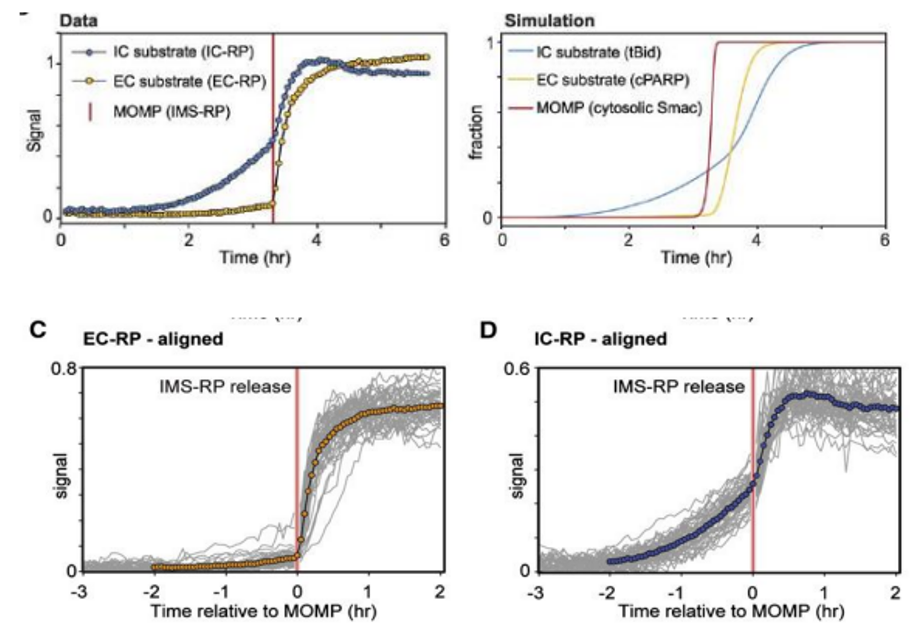
\includegraphics[width = 0.6\textwidth]{figs/simul-cells.png}
\end{figure}

En el artículo se ha estudiado el proceso de apoptosis de células tumorales tras administrar una droga (un fármaco). Las proteínas se han marcado fluorescentemente, y se puede ver cómo cambian las distintas proteínas tras la administración. Esto se puede simular de forma precisa, pero estas simulaciones se corresponden a experimentos de los que se obtiene una media poblacional. Las proteínas individuales tienen fluctuaciones en el tiempo. Todas las fluctuaciones están promedidadas, por lo que el modelo de ecuaciones diferenciales determinista simula el promedio de las células. En los experimentos se mide la fluorescencia total en la célula, no su localización subcelular.

En algunos sistemas, como el desarrollo embrionario, las \textbf{coordenadas espaciales} son cruciales. Las células se diferencian según su posición, y los genes se expresan en "oleadas". Para modelar estos sistemas, se usan \textbf{ecuaciones diferenciales parciales (EDPs),} que consideran tanto el tiempo como el espacio.

\begin{figure}[h]
\centering
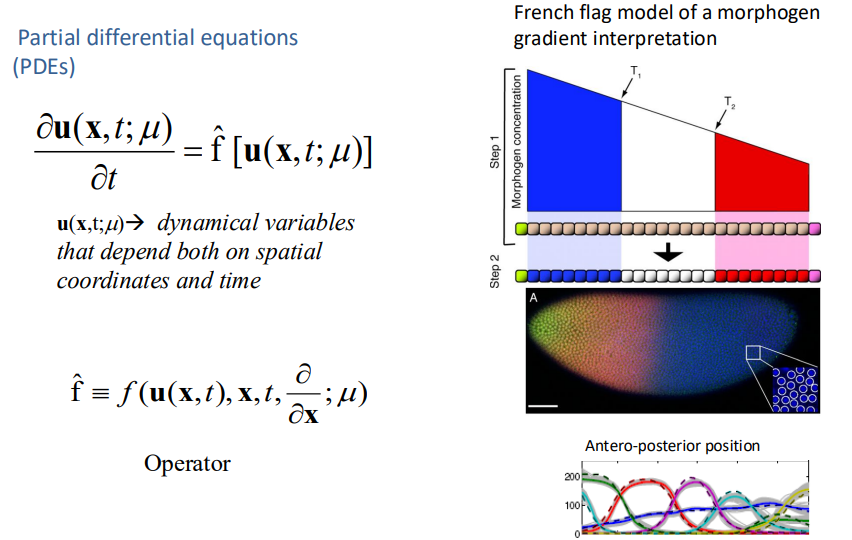
\includegraphics[width = 0.6\textwidth]{figs/pde-embryo.png}
\end{figure}

\section{Procesos dinámicos simples celulares: crecimiento celular, dilución proteica y degradación}
\subsection{Crecimiento celular}
El crecimiento celular es un proceso dinámico donde el número de células $N(t)$ aumenta con el tiempo. La velocidad de crecimiento se describe con la ecuación:
$$\frac{dN}{dt} = rN$$
donde r es la tasa de crecimiento y $N(t)$ el número de células en el tiempo t. Se trata de un sistema lineal con una sola variable. Los pasos para resolver la ecuación son:
\begin{enumerate}
\item Separar variables:
$$\frac{dN}{N} = r dt$$
\item Integrar ambos lados:
$$\int \frac{dN}{N} = \int r \cdot dt \rightarrow ln N = r t + C$$
\item Aplicar exponencial
$$N(t) = e^{rt + C} = e^C \cdot e^{rt}$$
\item Definir la constante $e^C = N(0)$, el número inicial de células o condiciones iniciales:
$$N(t) = N(0) \cdot e^{rt}$$
\end{enumerate}

El tiempo de duplicación $T_{div}$ indica el tiempo necesario para que $N(t)$ se duplique. Se calcula como:
$$N(T_{div}) = 2N(0) = N(0) \cdot e^{r \cdot T_{div}}$$
Dividiendo por $N(0)$:
$$ e^{r \cdot T_{div}} = 2 \rightarrow r \cdot T_{div} = ln 2 \rightarrow r = \frac{ln 2}{T_{div}}$$

\subsubsection{Ejercicio: Malthusian growth of bacteria}
Con el modelo lineal de crecimiento celular, ¿cuánto tiempo tardará una sola bacteria que se divide a un ritmo constante en llenar todos los océanos del mundo?. Datos: Supongamos que las bacterias tienen un volumen de 1 micrómetro cúbico y se dividen cada 30 minutos (valores típicos en \textit{E. coli}). El volumen estimado de todos los océanos es de $292.131.000 km^3$.

Podemos redondear el volumen de todos los océanos como:
$$V_{oceans} = 300.000.000 km^3 = 3 \cdot 10^8 km^3 = 3 \cdot 10^8 \cdot 10^{27} \mu m^3 = 3 \cdot 10^{35} \mu m^3$$
Los datos de una bacteria son:
$$V_{bacteria} = 1 \mu m^3$$
$$T_{div} = 30 mins = 0,5 h$$
Como partimos de una bacteria, la condición inicial es $c_0 = 1$.

Queremos que las bacterias colonicen todos los océanos. Para ello, se busca obtener el siguiente número de bacterias:
$$N = \frac{V_{oceans}}{V_{bacteria}} = \frac{3 \cdot 10^{35} \mu m^3}{1 \mu m^3} = 3 \cdot 10^{35}$$

Tenemos las siguientes fórmulas:
$$r = \frac{ln 2}{T_{div}} $$
$$N(t) = N(0) \cdot e^{rt} \rightarrow N(t) = e^{rt}$$

Sustituyendo, quedaría lo siguiente:
$$3 \cdot 10^{35} = e^{\frac{ln 2}{0,5} \cdot t} \rightarrow ln 3 + 35 \cdot ln 10 = \frac{ln 2}{0,5} \cdot t \rightarrow t = 58 h$$

Este modelo no es útil porque está demasiado simplificado. Hay que tener en cuenta los nutrientes, las restricciones espaciales, etc. 

%05/02 - Raúl Guantes
\subsection{Dilución proteica}
Durante el crecimiento celular, las proteínas se diluyen debido al aumento del volumen celular. Este fenómeno ocurre porque, al dividirse una célula, las proteínas se distribuyen entre las dos células hijas, reduciendo su concentración en cada una de ellas.

\subsubsection{Modelización de la dilución proteica}
Sea $P(t)$ el número de proteínas por célula en el tiempo $t$. Consideremos que partimos inicialmente de $P(0) = 8$ proteínas por célula y $N(0) = 1$ célula. 
Tras un tiempo de división $T_{div}$, la célula se divide en dos células hijas, y las proteínas se distribuyen aproximadamente en partes iguales entre ellas. Por tanto:
$$P(T_{div}) = \frac{P(0)}{2}$$
Tras $n$ divisiones celulares, el número de proteínas por célula se reduce a:
$$P(nT_{div}) = \frac{P(0)}{2^n}$$
Generalizando para cualquier tiempo $t$, el número de proteínas por célula sigue la relación:
$$P(t) = P(0) \cdot 2^{-\frac{t}{T_{div}}}$$

\subsubsection{Relación con el crecimiento exponencial de la población}
El número total de células $N(t)$ crece exponencialmente con el tiempo:
$$N(T_{div}) = N(0) \cdot e^{r \cdot T_{div}}$$
donde $r = ln 2 / T_{div}$ es la tasa de crecimiento. 

El número total de proteínas en la población $P^{tot}(t)$ se mantiene constante, ya que las proteínas no se crean ni se destruyen, solo se distribuyen entre las células hijas:
$$P^{tot}(t) = P^{tot}(0)$$
Por tanto, el número de proteínas por célula $P(t)$ se puede expresar como:
$$P(t) = \frac{P^{tot}(t)}{N(t)} = \frac{P^{tot} (0)}{N(0) \cdot e^{\frac{ln 2}{T_{div}} \cdot t}} = P(0) \cdot e^{-\frac{ln 2}{T_{div}} \cdot t}$$

\subsubsection{Ecuación diferencial de la dilución proteica}
La dinámica de la dilución proteica se describe mediante una ecuación diferencial que relaciona la tasa de cambio de $P(t)$ con el tiempo:
$$\frac{dP}{dt} = -\frac{ln 2}{T_{div}} \cdot P(t)$$

Es importante distinguir entre:
\begin{itemize}
\item \textbf{Ecuación diferencial:} describe cómo cambia $P(t)$ con el tiempo. En este caso, indica que la tasa de cambio de $P(t)$ es proporcional a $P(t)$ misma, con una constante de proporcionalidad negativa $- ln 2/T_{div}$.
\item \textbf{Solución de la ecuación diferencial:} proporciona la expresión explícita de $P(t)$ en función del tiempo.
\end{itemize}

En este contexto de dilución proteica, la tasa de cambio de la cantidad de proteínas por célula $P(t)$ se puede expresar en términos de una \textbf{constante de dilución} $\delta_{dil}$, definida como:
$$ \delta_{dil} = \frac{ln 2}{T_{div}}$$
Por lo tanto, la ecuación diferencial que describe la dilución proteica se reescribe como:
$$\frac{dP}{dt} = -\frac{ln 2}{T_{div}} \cdot P(t) = -\delta_{dil} \cdot P(t)$$
Esta ecuación indica que la cantidad de proteínas por célula disminuye exponencialmente con el tiempo debido a la división celular.

\subsection{Degradación activa de proteica}
Además de la dilución, las proteínas también pueden sufrir degradación activa, un proceso en el que las proteínas son descompuestas o eliminadas de la célula. En aproximadamente el 80\% de los casos medidos, la cantidad de proteínas disminuye de forma exponencial debido a este proceso.

\subsubsection{Modelización de la degradación}
La degradación activa se modela mediante una tasa de degradación $\delta_{deg}$, que describe cómo la cantidad total de proteínas $P^{tot}(t)$ en la población celular disminuye con el tiempo:
$$P^{tot}(t) = P^{tot}(0) \cdot e^{-\delta_{deg}\cdot t}$$

La ecuación diferencial que describe este proceso es:
$$ \frac{dP^{tot}}{dt} = -\delta_{deg} \cdot P^{tot}$$

\subsubsection{Combinación de dilución y degradación}
Cuando tanto la dilución como la degradación están presentes, la cantidad de proteínas por célula $P(t)$ se ve afectada por ambos procesos. Para modelar esto, combinamos las contribuciones de la dilución y la degradación.
\begin{enumerate}
\item \textbf{Cantidad total de proteínas}
$$P^{tot}(t) = P^{tot}(0) \cdot e^{-\delta_{deg} \cdot t}$$

\item \textbf{Número de células}
$$N(t) = N(0) \cdot e^{\frac{ln 2}{T_{div}} \cdot t}$$

\item \textbf{Proteínas por célula}
$$P(t) = \frac{P^{tot} (t)}{N(t)} = \frac{P^{tot}(0) \cdot e^{-\delta_{deg} \cdot t}}{N(0) \cdot e^{\frac{ln 2}{T_{div}} \cdot t}} = P(0) \cdot e^{-(\delta_{deg} + \frac{ln2}{T_{div}})t}$$
donde $P(0) = \frac{P^{tot}(0)}{N(0)}$ es la cantidad inicial de proteínas por célula.

\item \textbf{Tasa de cambio combinada}

Definimos la \textbf{tasa de disminución total} $\delta$ como la suma de la tasa de degradación activa $\delta_{deg}$ y la tasa de dilución $\delta_{dil}$:
$$\delta = \delta_{deg} + \delta_{dil}$$
Por tanto, la expresión para $P(t)$ se simplifica a:
$$P(t) = P(0) \cdot e^{-\delta \cdot t}$$
Y la ecuación diferencial que describe la dinámica combinada es:
$$\frac{dP}{dt} = -\delta P$$
\end{enumerate}

La constante $\delta$ representa la tasa efectiva de disminución de proteínas por célula, teniendo en cuenta tanto la degradación activa como la dilución debida al crecimiento celular. Un valor mayor de $\delta$ indica una disminución más rápida de la cantidad de proteínas por célula.

\subsubsection{Vida media}
La vida media ($T_{1/2}$) es el tiempo necesario para que la concentración de una sustancia (en este caso, proteínas) se reduzca a la mitad de su valor inicial. Matemáticamente, esto se expresa como:
$$P(T_{1/2}) = \frac{P(0)}{2}$$

Partiendo de la ecuación que describe la disminución exponencial de la concentración de proteínas:
$$P(t) = P(0) \cdot e^{-\delta t}$$
Sustituyendo $t = T_{1/2}$ y $P(T_{1/2}) = \frac{P(0)}{2}$, obtenemos:
$$\frac{P(0)}{2} = P(0) \cdot e^{-\delta \cdot T_{1/2}}$$
Simplificando $P(0)$ en ambos lados:
$$\frac{1}{2} = e^{-\delta \cdot T_{1/2}}$$
Aplicando el logaritmo neperiano a ambos lados:
$$ln(\frac{1}{2}) = - \delta \cdot T_{1/2}$$
Resolviendo para $T_{1/2}$:
$$T_{1/2} = \frac{ln 2}{\delta}$$
Por lo tanto, la constante de disminución $\delta$ se relaciona con la vida media mediante:
$$\delta = \frac{ln 2}{T_{1/2}}$$

\subsection{Combinación: producción y degradación de proteínas}
En muchos sistemas biológicos, las proteínas no solo se degradan, sino que también se producen activamente. Para modelar este proceso, introducimos:
\begin{itemize}
\item $\alpha$: la \textbf{tasa de producción} de proteínas, con unidades de proteínas por unidad de tiempo.
\item $\delta$: la \textbf{tasa de disminución total}, que incluye tanto la degradación activa como la dilución debida al crecimiento celular, con unidad de inversa de tiempo.
\end{itemize}
La dinámica de la cantidad de proteínas $P(t)$ se describe mediante la siguiente ecuación diferencial:
$$\frac{dP}{dt} = \alpha - \delta P$$

\subsubsection{Resolución de la ecuación diferencial}
Para resolver esta ecuación, seguimos los siguientes pasos:
\begin{enumerate}
\item \textbf{Separación de variables}
$$\frac{dP}{\alpha - \delta P} = dt$$

\item \textbf{Integración de ambos lados}
$$\int \frac{dP}{\alpha - \delta P} = \int dt$$

\item \textbf{Resolución de las integrales}

La integral del lado derecho es:
$$\int dt = t + cte$$

La integral del lado izquierdo requiere una sustitución. Sea $u = \alpha - \delta P$, entonces $du = - \delta dP$, y
$$\int \frac{dP}{\alpha - \delta P} = - \frac{1}{\delta} \int \frac{du}{u} = -\frac{1}{\delta} ln |u| + C = -\frac{1}{\delta} ln(\alpha - \delta P) + C$$

\item \textbf{Igualando ambas integrales}
$$-\frac{1}{\delta} ln (\alpha - \delta P) = t + C$$

\item \textbf{Despejando $P(t)$}

Multiplicamos ambos lados por $-\delta$:
$$ln(\alpha - \delta P) = -\delta t + C'$$
donde $C' = -\delta C$.

Aplicamos la exponencial a ambos lados:
$$\alpha - \delta P = e^{-\delta t + C'} = e^{C'} \cdot e^{-\delta t}$$

Despejamos $P(t)$:
$$P(t) = \frac{\alpha}{\delta} - \frac{e^{C'}}{\delta} e^{-\delta t}$$

\item \textbf{Determinación de la constante $C'$}

Aplicamos la condición inicial $P(0)$:
$$P(0) = \frac{\alpha}{\delta} - \frac{e^{C'}}{\delta}$$

Despejamos $e^{C'}$:
$$e^{C'} = \alpha - \delta P(0)$$

\item \textbf{Sustituyendo $e^{C'}$ en la solución}:
$$P(t) = \frac{\alpha}{\delta} - \frac{\alpha - \delta P(0)}{\delta} e^{-\delta t}$$
Y simplificando:
$$P(t) = \frac{\alpha}{\delta} (1 - e^{-\delta t}) + P(0) e^{-\delta t}$$
\end{enumerate}

\subsubsection{Estado estacionario}
Cuando $t\rightarrow \infty$, el término exponencial $e^{-\delta t}$ tiende a 0, y la cantidad de proteínas $P(t)$ alcanza un estado estacionario:
$P(t) \rightarrow \frac{\alpha}{\delta}$
Este valor representa el equilibrio entre la producción y la degradación de proteínas.




%05/02 - Raúl Guantes
\chapter{Sistemas dinámicos no lineales}
\section{Crecimiento logístico}
El crecimiento de las poblaciones está limitado por los recursos que están disponibles. Para ello, se debe añadir un parámetro nuevo, denominado como $k$, que indica la cantidad de recursos. Suponemos que la población tiene una tasa de crecimiento $r$ positiva. Además, contamos con $N(t)$, que es el número de células a un tiempo t. 

Suponiendo que hay una ecuación diferencial que dice cómo cambia la población con el tiempo en función de la variable y los parámetros r y k:
$$\frac{dN}{dt} = f(N; r, k)$$
Suponiendo que los recursos son ilimitados, $r N$. No obstante, si los recursos son limitados, entonces el tamaño depende de los recursos. Si la población es mayor que la disponibilidad de los recursos, la población debe disminuir y habrá células que mueran. SI el tamaño de la población es pequeño, hay recursos suficientes y la población crece. En otras palabras, la derivada es positiva o negariva según si la población crece o disminuye respectivamente. 
$$r N (1 - \frac{N}{k}$$
Esto se conoce como la ecuación de crecimiento logística. Esta ecuuación es no lineal porque N termina estando al cuadrado. 

$$N(t) = \frac{N(0) k}{N(0) + (k - N(0))e^{-rt}}$$
A tiempo infinito, la población tiende al valor de k, quedando en el equilibrio.
En estado de equilibrio, la derivada en función del tiempo da 0. 
$$0 = r N (1 - \frac{N}{K}) \begin{cases} 
N^1_{eq} = K \rightarrow \text{Estable} \\
N^2_{eq} = 0 \rightarrow \text{Inestable}
\end{cases}
$$

Para entender el comportamiento a tiempos largos (en equilibrio), hay que calcular puntos de equilibrio y la estabilidad. Si tenemos un sistema biológico de verdad, al medir a tiempos largos, siempre va a estar en un estado de equilibrio estable, al ser robustos a fluctuaciones. La estabilidad se puede deducir sin resolver la ecuación diferencial mediante dos formas: la forma gráfica y la forma matemática. 

\subsection{Cálculo de estabilidad de forma gráfica}
Con una sola variable, se pinta el denominado \textbf{plano de fases}. En el eje x está la variable, y en el y la derivada de la variable con respecto al tiempo. 
$$\frac{dN}{dt} = f(N) = rN - \frac{rN^2}{K}$$ 
Los puntos de corte son en 0 y en k, quedando una parábola invertida. Para calcular el máximo hay que poner la derivada en 0.
$$\frac{df}{dN} = 0 = r - \frac{2rN}{k} \rightarrow N = \rightarrow N = \frac{rk}{2r} = \frac{k}{2}$$

El punto de equilibrio en k es estable, porque N siempre va a converger a ese punto, ya que en un lado la función es positiva y en el otro lado negativa.

\subsection{Cálculo de estabilidad de forma matemática o por linealización}
La ventaja de este método es que se puede aplicar al número de variables que se quiera. Esta estabilidad se obtiene por linealización. 
Se busca analizar la función en un valor de equilibrio con una pequeña perturbación. 
$$N = N_{eq} + \Delta N$$
Al derivar:
$$\frac{d(N_{eq} + \Delta N)}{dt} = f(N_{eq} + \Delta N$$
$$(\frac{dN_{eq}}{dt} = 0) + \frac{d \Delta N}{dt}$$

$f(N)$ se aproxima por un polinomio según la serie de Taylor. En otras palabras, se aproxima:
$$f(N) \approx a + bN + cN^2 + dN^3 + \ldots$$ 
Vamos a usar eso para realizar una aproximación alrededor de un punto $N_0$. Para aproximar en una línea recta, debe pasar por ese punto y su pendiente debe ser la pendiente de la función, es decir, la derivada de la función y la variable.
$$a = f(N_0); b = \frac{df}{dN}; f = a + bN$$

$$f(N) \approx f(N_0) + \frac{df(N_0)}{dN} (N-N_0) + \frac{1}{2} \frac{d^2f(N_0)}{dN^2} (N-N_0)^2 + \ldots \frac{1}{n!} \frac{d^n(N_0)}{dN^n}(N-N_0)^n$$
Esta aproximación de Taylor se utiliza para aproximar la función $f(N_{eq} + \Delta N$ alrededor del punto $N_{eq}$. 
$$\frac{d \Delta N}{dt} = f(N_{eq} + \frac{df(N_{eq})}{dN} (N-N_{eq}) \rightarrow \frac{\Delta N}{dt} = f'(N_{eq} \Delta N$$

Si $f'(N_{eq}) > 0$, el punto de equilibrio es inestable, ya que aumentaría en el tiempo ($\Delta N(t) = \Delta N(0) \cdot e^{f'(N_{eq}) t}$). Si $f'(N_{eq}) < 0$, entonces el punto de equilibrio es estable.


%27/02 - Raúl Guantes
\chapter{Redes biológicas y modelos de redes reguladoras}
\section{Redes complejas en biología}
Históricamente, las primeras redes que se caracterizaron al completo fueron la red del factor de transcripción de \textit{Escherichia coli} y las redes de interacción proteica en \textit{Saccharomyces cerevisiae}. Actualmente hay muchas bases de datos con las redes de muchos organismos. También hay redes neuronales de C. elegans. 

Las redes biológicas pueden representarse como «grafos» con nodos y conexiones. Cada nodo representa un elemento de la red, y las conexiones representan las interacciones entre los elementos.
Por ejemplo, la red de interacción de proteínas tiene un nodo para cada proteína y conexiones entre las proteínas que interaccionan entre sí. 

Analizando la estructura de la red y las conexiones entre los nodos podemos extraer algunas conclusiones sobre algunos «principios de diseño» biológicos:
\begin{itemize}
\item \textbf{Redes aleatorias:} las conexiones son equiprobables y aleatorias entre los nodos.
\item \textbf{Redes libres de escala:} hay unos ciertos nodos con más probabilidad de conexión que otros y que se denominan hubs. 
\item \textbf{Redes jerárquicas}
\end{itemize}

Las redes modernas en biología son:
\begin{itemize}
\item \textbf{Redes dinámicas o de evolución temporal}: las conexiones varían en el tiempo. Por ejemplo, la expresión de genes en una célula depende de perturbaciones. Los nodos se mantienen, pero son las conexiones las que van cambiando. 
\item \textbf{Redes multicapa:} hay diferentes tipos de redes que pueden interaccionar entre sí. Un ejemplo: en ecología hay muchas redes multicapa si se analizan las interacciones de virus y huéspedes. Una capa puede ser todos los tipos de virus, otra los tipos de plantas o huéspedes, otra con los distintos ambientes, etc. Otro ejemplo es una red de interacción de proteínas del virus con las proteínas del huésped. Las redes tienen distintas estructuras, dando lugar a un cierto tipo de dinámica entre esa red.
\item \textbf{Redes neuronales multiescala:} un ejemplo es la red neuronal que salió a finales de 2024 con la reconstrucción del cerebro completo de una mosca adulta. 
\end{itemize}

Para extraer información de las redes, primero se puede mirar la estructura que tiene. Una forma de ver si tiene una estructura especial es comparar la red con una aleatoria. Para el mismo número de nodos y conexiones, se reconecta la red al azar con equiprobabilidad. En la red real, se pueden describir hubs que están más conectadas. 

En biología, las redes suelen ser libres de escala y modulares. Estas redes son más robustas, es decir, si se elimina un nodo, la estructura no se perturba tanto o no colapsa. A esto se le conoce como \textbf{principio de robustez}.

\begin{figure}[h]
\centering
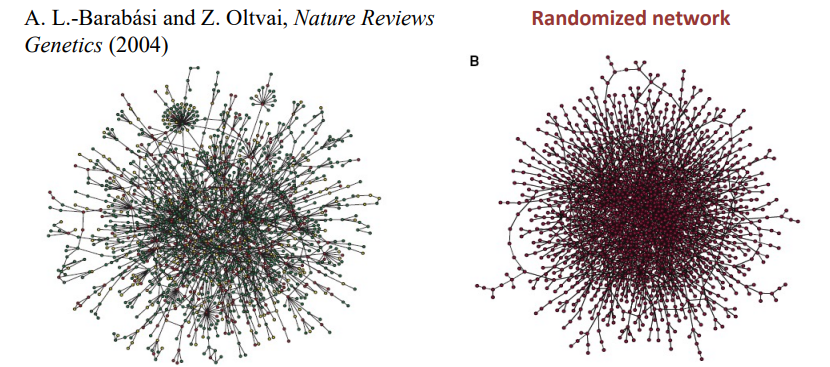
\includegraphics[width = 0.7\textwidth]{figs/biological-network.png}
\end{figure}

\section{Modularidad: motivos de redes}
Cuando se empezaron a estudiar las redes biológicas, se empezó a ver que la estructura de redes biológicas cambia la idea de la evolución de los sistemas biológicos. Como dijo François Jacob, 
\begin{quotation}
La naturaleza funciona por integración. Cualquiera que sea el nivel, los objetos analizados por las ciencias naturales son siempre organizaciones, o sistemas. Cada sistema de un nivel determinado utiliza como ingredientes algunos sistemas del nivel más simple, pero sólo algunos.
\end{quotation}

Algunos patrones dentro de una red compleja aparecen con mucha más frecuencia que otros (principio de recurrencia). Estos patrones se denominan \textbf{motivos o módulos de red}.

\begin{figure}[h]
\centering
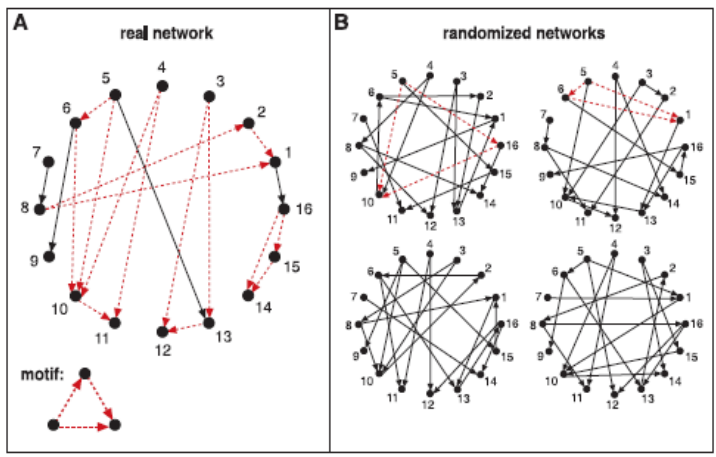
\includegraphics[width = 0.7\textwidth]{figs/motivo-redes.png}
\end{figure}

¿Los motivos de red representan entidades funcionales útiles? La biología de sistemas intentaba comprender la red biológica mediante representaciones más sencillas. 

\section{Redes de regulación transcriptómica}
En una red reguladora, los «nodos» son factores de transcripción. La actividad de cada gen viene dada por el nivel de proteína producida en un momento dado. 

La siguiente red fue construida en 2008 para representar todos los factores de transcripción que participan en el desarrollo embrionario humano. Mirando en detalle las conexiones entre los factores de transcripción, hay muchos motivos de retroalimentación: un nodo afecta a un segundo nodo, el cual a su vez afecta al primero, y cada uno de ellos tiene su propia retroalimentación. 

\begin{figure}[h]
\centering
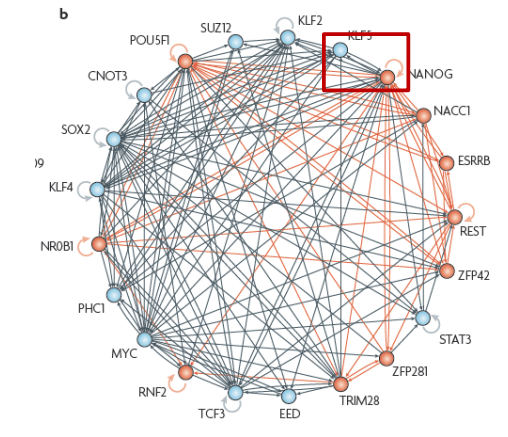
\includegraphics[width = 0.7\textwidth]{figs/red-embrionaria.png}
\end{figure}

La dinámica simple de nacimiento/muerte de una proteína Y que estudiamos (producción constante y degradación lineal) puede representarse mediante las reacciones bioquímicas: 
$$\frac{dY}{dt} = \alpha - \delta Y$$
Esto se considera en el modelo de la siguiente forma:
\begin{figure}[h]
\centering
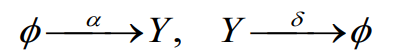
\includegraphics[width = 0.7\textwidth]{figs/reacciones.png}
\caption{Las proteínas Y se crean mediante $\alpha$, y desaparecen mediante $\delta$.}
\end{figure}

Algunas proteínas actúan como factores de transcipción, activando o reprimiendo la expresión de otra proteína. 

¿Cuánta proteína Y se produce en función de la cantidad de X que hay?
\begin{figure}[h]
\centering
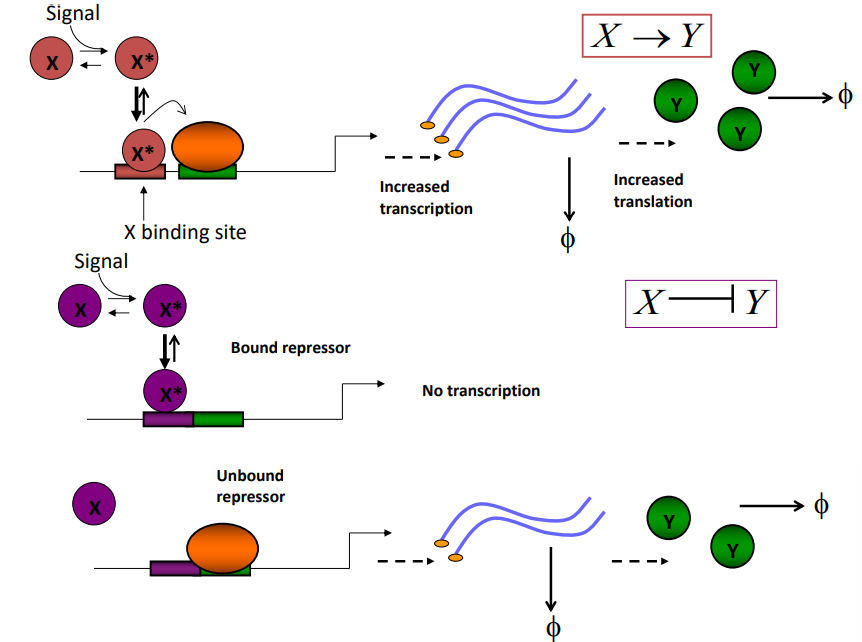
\includegraphics[width = 0.7\textwidth]{figs/factores-transcripcion.png}
\caption{Las proteínas activas se marcan con un asterisco. Cuando X es un activador, al unirse se favorece la transcripción de Y, aumentando su cantidad. Cuando X es un inhibidor, al unirse al gen no se produce la transcripción (no se genera Y).}
\end{figure}

Vamos a analizar esto de forma matemática.
\begin{enumerate}
\item \textbf{Escribir todas las especies (variables) de interés y las reacciones bioquímicas en las que interviene cada especie:}
\begin{itemize}
\item X: factor de transcripción inactivo
\item X*: factor de transcripción activo
\item P: promotor del gen Y libre
\item PX*: promotor del gen Y unido a X*
\item M: mRNA
\item Y: proteína resultante
\end{itemize}
Normalmente los factores de transcripción son activos cuando forman oligómeros (dos o más moléculas de X se asocian formando un complejo).

\item \textbf{Analizar las distintas reacciones o interacciones entre las variables:}
\begin{enumerate}
\item Activación / desactivación del factor de transcripción X. Esto se puede hacer por fosforilación o formación de complejos (oligómeros). 
$$nX \xrightarrow{K_a} X_n$$
$$X_n \xrightarrow{K_d} nX$$
siendo $K_a$ la constante de asociación y $K_d$ la constante de disociación.

\item Unión y desunión del factor de transcripción X al promotor P.
$$P + X_n \xrightarrow{K_b} (PX_n)$$
$$(PX_n) \xrightarrow{K_u} P + X_n$$
siendo $K_b$ la constante de unión (binding) y $K_u$ la constante de unbinding. 

\item Transcripción

Si es del promotor libre, da lugar al mRNA con una constante de transcripción $\beta$. Esto se da por ejemplo cuando X es un inhibidor y no está unido.
$$P \xrightarrow{\beta} P + M$$

Si X es un activador y está unido, la reacción se describe con la tasa de transcripción $\rho$:
$$(PX_n) \xrightarrow{\rho} (PX_n) + M$$

Si $\beta$ es mayor que $\rho$, X es un represor al haber más expresión si el factor de transcripción no está ligado. Si $\beta$ es menor que $\rho$, X es un activador, aumentando la expresión de la proteína tras la unión de X. 

\item Traducción
$$M \xrightarrow{\alpha} M + Y$$

\item Degradación de ARNm y proteínas con su velocidad de degradación $\delta$.
$$M \xrightarrow{\delta_M} \varnothing$$
$$Y \xrightarrow{\delta_Y} \varnothing$$
\end{enumerate}

\item \textbf{Considerar restricciones o ligaduras}
Una relación entre variables obvia es que, si la célula no se está dividiendo, el gen sólo puede estar en dos estados: libre u ocupado, por lo que su número de copias es constante.
$$P + PX_n = P^T (constante)$$

\item \textbf{Escribir la evolución temporal de cada especie utilizando la ley de acción de masas}
Ley de acción de masas dice que las velocidades de reacción son proporcionales a los productos de las concentraciones de reactivos.
La ecuación de ganancia/pérdida se describe como $dx/dt = production - degradation$. 

\begin{equation}
\tag{a}
\frac{dX}{dt} = nK_d \cdot X_n - nK_a \cdot X^n
\end{equation}
\begin{equation}
\tag{a,b}
\frac{dX_n}{dt} = K_a \cdot X^n + K_u \cdot (PX_n) - K_d \cdot X_n - K_b \cdot P \cdot X_n
\end{equation}
\begin{equation}
\tag{b}
\frac{dP}{dt} = K_u \cdot (PX_n) - K_b \cdot P \cdot X_n
\end{equation}
\begin{equation}
\tag{c}
\frac{d(PX_n)}{dt} = K_b \cdot P \cdot X_n - K_u \cdot (PX_n)
\end{equation}
\begin{equation}
\tag{c,e}
\frac{dM}{dt} = \beta P + \rho (PX_n) - \delta_M M
\end{equation}
\begin{equation}
\tag{d,e}
\frac{dY}{dt} = \alpha M - \delta_Y Y
\end{equation}

\item \textbf{Considerar las escalas temporales de las diferentes reacciones}
El problema de las constantes es que no se conocen. Una aproximación para simplificar las constantes es mediante agrupación de escalas temporales. La activación de un factor de transcripción tarda un milisegundo, y la unión de dicho factor a su sitio del ADN un segundo. Estos son reacciones rápidas. Por el contrario, la transcripción y traducción de un gen dura 5 minutos, y la degradación proteica dura hasta 1 hora, siendo reacciones lentas. Así, suponemos que las reacciones rápidas están en equilibrio con respecto a las lentas, y no las consideramos como variables dinámicas.
$$\frac{dX}{dt} = nK_dX_n - nK_aX^n \cong 0 \rightarrow \frac{X_n}{X^n} = \frac{K_a}{K_d} \equiv K_{act}$$
Definir de este modo las constantes de equilibrio para todas las reacciones rápidas permite eliminar variables. Por ejemplo, se puede expresar $X_n$ como:
$$X_n = K_{act} X^n$$
y, del equilibrio de unión y desunión al promotor, la variable del promotor ocupado se puede definir como:
$$(PX_n) =  \frac{K_b}{K_u} \cdot P \cdot X_n = K_{bind} \cdot P \cdot X_n = K_{bind} k_{act} P \cdot X^n = K_x P \cdot X^n$$
El último paso consiste en expresar la variable promotora libre P, que es una variable rápida, en función de la cantidad del factor de transcripción X. Utilizando la restricción $P + (PX_n) = 1$, obtenemos:
$$P + (PX_n) = 1 = P(1 + K_xX^n) \rightarrow P = \frac{1}{1 + K_xX_n}$$
De esta forma, eliminamos las ecuaciones para las variables rápidas, manteniendo sólo la dinámica del ARNm y de las proteínas, y expresando todas las variables rápidas en estas ecuaciones restantes como una función de X:
$$\frac{dY}{dt} = \alpha M - \delta_Y Y$$
$$\frac{dM}{dt} = \beta \frac{1}{1 + K_xX^n} + \rho \frac{K_xX^n}{1 + K_x X^n} - \delta_M M$$

Si asumimos que la transcripción de Y solo es posible cuando el factor de transcripción está unido:
$$\frac{dM}{dt} = \rho \frac{X^n K_x}{1 + X^nK_x} - \delta_M M$$

\item \textbf{Suposición del estado cuasi estacionario para el ARNm}
Cuando la degradación del ARNm ocurre mucho más rápido que la degradación proteica ($\delta_M >> \delta_Y$), entonces se puede suponer que: 
$$\frac{dM}{dt} \approx 0 \rightarrow \frac{dY}{dt} = \sigma_{act} \frac{X^n K_x}{1 + X^n K_x} - \delta_Y Y$$

Así, podemos expresar cómo cambia la concentración de equilibrio de nuestra proteína Y en función de la cantidad de X (nuestra «entrada») en términos de una función de Hill (también llamada función de respuesta, función de regulación o relación entrada/salida):
$$f(x) = \frac{(X/\theta)^n}{1 + (X/\theta)^n}$$

\begin{figure}[h]
\centering
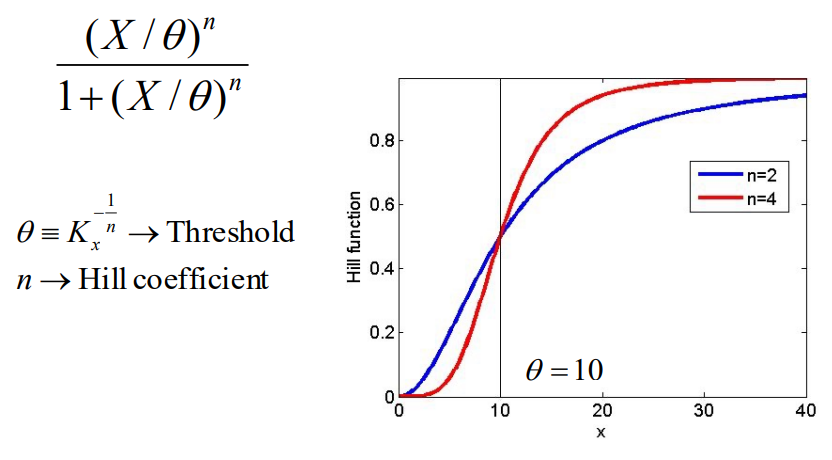
\includegraphics[width = 0.6\textwidth]{figs/hill-function.png}
\end{figure}
Para $n \rightarrow \infty$, se produce una función escalón. En este caso, n representa la cooperatividad, el número de oligomerización o fosforilaciones necesarias para que funcione. Proporciona la pendiente de la subida. $\theta$ representa el umbral de producción.

Si asumimos que la transcripción del gen Y solo se puede dar cuando el promotor está libre, entonces
$$\frac{dY}{dt} = \sigma_{rep} \frac{1}{1 + X^n K_x} - \delta_Y Y$$
y se representa en la función represora de Hill.

\begin{figure}[h]
\centering
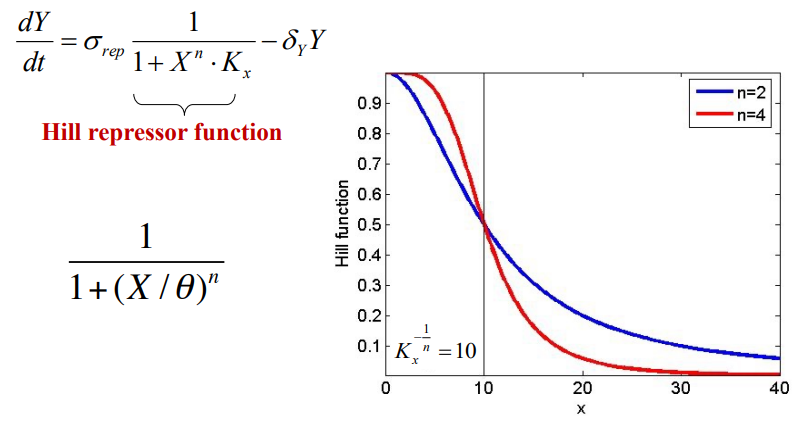
\includegraphics[width = 0.6\textwidth]{figs/hill-function-rep.png}
\end{figure}

En resumen, las interacciones entre genes pueden cuantificarse mediante funciones sigmoidales (Hill) con dos parámetros (umbral de activación/represión y cooperatividad).
\end{enumerate}

Puede haber casos donde haya varios reguladores para una proteína, siendo esto muy frecuente en eucariotas. Cuando hay varios inputs que están activando al mismo nodo, puede haber muchas combinaciones posibles del efecto de esos inputs. 

\begin{figure}[h]
\centering
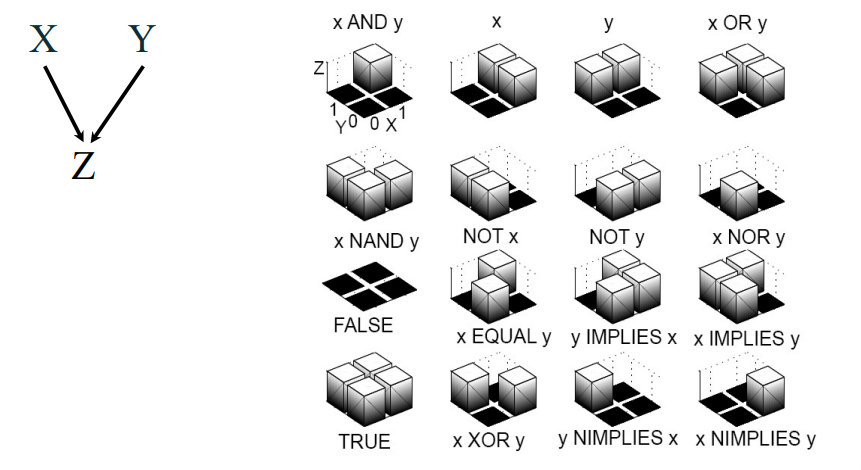
\includegraphics[width = 0.8\textwidth]{figs/logic-gates.png}
\end{figure}

Una puerta de tipo AND se puede representar de la siguiente forma:
$$f(x,y) = \frac{(X/K_x)^n}{1 + (X/K_x)^n} \times \frac{(Y/K_y)^n}{1 + (Y/K_y)^n}$$

En el caso de una puerta OR:
$$f(x,y) = \frac{(X/K_x)^n}{1 + (X/K_x)^n} + \frac{(Y/K_y)^n}{1 + (Y/K_y)^n}$$

\section{Función de motivos de redes en redes reguladoras}
Los bucles de retroalimentación se dan cuando hay una interacción de X a Y y de Y a X. Para ver cómo es la retroalimentación, se debe multiplicar el efecto de todas las interacciones (ver si un bucle es positivo o negativo).

Se distinguen los feedforward loops (FFL) coherentes, donde una interacción y otra tienen el mismo efecto, de los FFL incoherentes donde hay efectos contrarios.

\subsection{Motivo de red más simple: autorregulación}
El motivo de red más simple es el de un gen autoregulado, ya sea de forma positiva o negativa. En \textit{E. coli}, hay 400 nodos y 500 enlaces. Por azar, esperaríamos que hubiese 1,2 autorfegulaciones (500/400). Como se trata de una distribución independiente de Poisson, realmente es de $1.2 \pm \sqrt{1.2}$. De forma experimental, se encontraron 40 autorregulaciones negativas, siendo esto mucho mayor de lo esperado.

Suponemos que hay un gen que produce la proteína Y a partir de una señal con velocidad $\alpha$ y se degrada en $\delta$. 
$$\frac{dY}{dt} = \alpha - \delta Y$$

¿Cuál es el tiempo de respuesta a la señal? El tiempo de respuesta se considera que es la mitad del valor estacionario $\alpha/\delta$. Como la función se describe con la fórmula
$$Y(t) = \frac{\alpha}{\delta} (1 - e^{-\delta t})$$
el tiempo de respuesta se calcularía de la siguiente forma:
$$Y(t-T_{resp}): \frac{\alpha}{2 \delta} = \frac{\alpha}{\delta} (1 - e^{-\delta T_{resp})}$$
teniendo que despejar $T_{resp}$.

%06/03 - Raúl Guantes
El tiempo de respuesta de un gen es el tiempo necesario para llegar a la mitad de la respuesta total:
$$T_{1/2} = \frac{\ln 2}{\delta}$$
Si la proteína es estable y sólo se degrada por dilución, entonces $T_{1/2} = T_{div}$. Esto es un proceso muy lento. Para poder aumentar su velocidad, se podría aumentar $\delta$, teniendo que aumentar por consiguiente también $\alpha$. 

\subsubsection{Autorregulación negativa}
Considerando un gen con autorregulación negativa, cambia en el tiempo con el término
$$\frac{dY}{dt} = f(Y) - \delta Y$$
siendo $f(Y)$ la tasa de producción y $\delta Y$ la tasa de degradación. Como es una autorregulación negativa, $f(Y)$ tendrá la forma de una sigmoidal negativa (por ejemplo, $f(Y) = \frac{1}{1 + (Y/k)^2}$. El valor de equilibrio se dará cuando $f(Y) = \delta Y$. La gráfica que define esto se denomina como gráfica del balance de tasas o rate balance plot:
\begin{figure}[h]
\centering
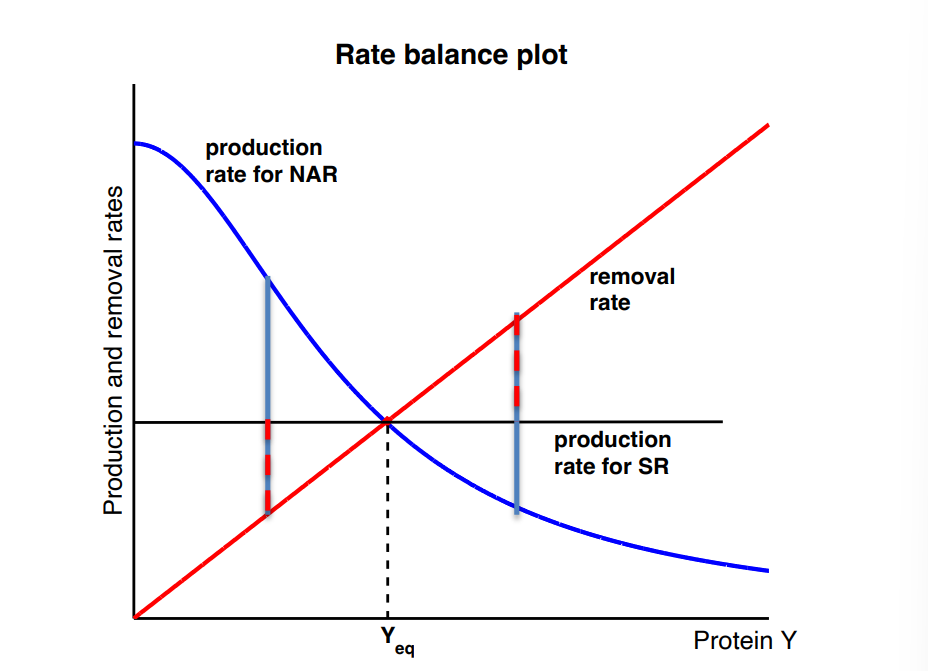
\includegraphics[width = 0.6\textwidth]{figs/rate-balance-plot.png}
\end{figure}

Al calcular la derivada, se vería que ese punto de equilibrio sería estable, el cual depende del umbral de represión $Y/k$ que biológicamente depende de la afinidad de la proteína por el promotor. El tiempo de respuesta depende de la magnitud de la derivada; cuanto mayor sea en valor absoluto, mayor velocidad de cambio.

Para un modelo sin regulación (producción constante):
$$\frac{dY}{dt} = \alpha - \delta Y$$
Para comparar los tiempos de respuesta, se debe comparar el valor absoluto de la derivada.
\begin{itemize}
\item $Y < Y_{eq}$: la tasa de cambio de la autorregulación negativa es más grande que la tasa de cambio de la regulación simple.
\item $Y > Y_{eq}$: el valor absoluto de la tasa de cambio de la autorregulación negativa es mayor que el valor absoluto de la tasa de cambio de la regulación simple. 
\end{itemize}

La autorregulación negativa acelera el tiempo de respuesta.
\begin{figure}[h]
\centering
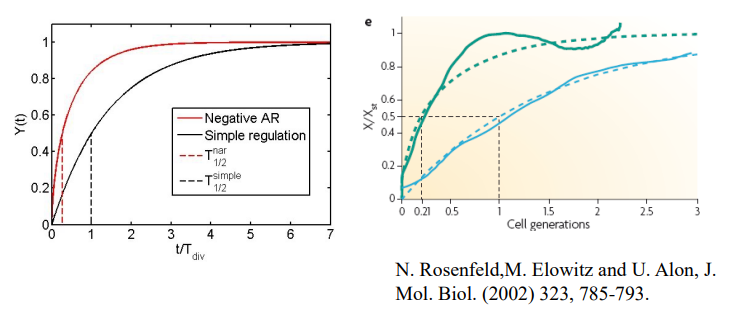
\includegraphics[width = 0.8\textwidth]{figs/nar.png}
\end{figure}

\subsubsection{Autorregulación positiva}
Para una autorregulación positiva, la proteína se describe con la misma función:
$$\frac{dY}{dt} = f(Y) - \delta Y$$
Ahora, $f(Y)$ es creciente con forma de función de Hills, mientras que la tasa de degradación sigue con una forma de recta. El punto en el que se cortan es el punto de equilibrio, el cual es estable. En este caso, el valor absoluto de la derivada del modelo sin regulación es mayor que el valor de la derivada del modelo con autorregulación positiva. Por tanto, la autorregulación positiva aumenta el tiempo de respuesta (es más lento). 
\begin{figure}[h]
\centering
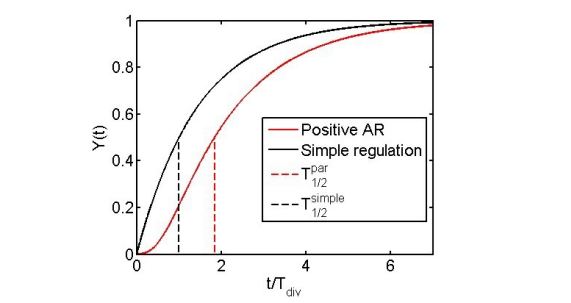
\includegraphics[width = 0.8\textwidth]{figs/par.png}
\end{figure}

Tanto la producción como el ciclo celular tienen fluctuaciones, por lo que necesita genes que respondan más rápido y más lentamente. Si $\delta$ cambia, la función de degradación cambia, teniendo mayor o menor pendiente. Cuando hay producción constante, el valor de equilibrio se mueve, mientras que la tasa de producción con autorregulación negativa apenas se ve modificada. Por tanto, la autorregulación negativa produce resistencia frente a fluctuaciones en producción $\alpha$ o en tiempos de división $\delta$. 

Si la función de autorregulación más suave ($f(Y) = \frac{(Y/k)^n}{1 + (Y/k)^n}$), entonces habrá más puntos de equilibrio. El punto de equilibrio en 0 es estable, al igual que aquel en el que la producción de proteína se satura. Entre ellos, debe haber un punto de equilibrio inestable, el cual separa las condiciones iniciales. Por tanto, tenemos un modelo de biestabilidad con dos estados posibles: $Y_{eq} = 0, Y_{eq}^{max}$. Todo esto se produce si $f(Y)$ es cooperativo. 

Poniendo un ejemplo concreto, suponemos que $n = 2$ y que $k = 1$. Por tanto, el modelo que tenemos es:
$$\frac{dY}{dt} = s + \frac{Y^2}{1 + Y^2} - \delta Y$$
siendo $s$ las señales bioquímicas. 

Si no hay señales bioquímicas ($s=0$), los puntos de equilibrio se deben calcular de la siguiente forma:
$$Y \frac{Y}{1 + Y^2} = \delta Y \begin{cases}
Y^1_{eq} = 0 \\
\frac{Y}{1 + Y^2} = \delta
\end{cases}
$$
$$\delta Y^2_{eq} + \delta - Y_{eq} = 0$$
$$Y_{eq} = \frac{1 \pm \sqrt{1 - 4 \delta^2}}{2}$$
$$1 - 4 \delta^2 > 0 $$
$$4 \delta^2 < 1$$
$$\delta < 1/2$$

Por tanto, hay tres puntos de equilibrio, los cuales causan la bifurcación silla-nodo. 

Añadiendo un inductor ($s$), la recta de degradación se desplaza hacia los lados desde el origen. Para un $\delta = 0.55$ y $s=0$, no hay producción. No obstante, cuando $s = 0.2$, la producción basal aumenta la producción de la proteína, viéndose amplificada por la autorregulación positiva. Esto se conoce como \textbf{interruptor genético}.  

\begin{figure}[h]
\centering
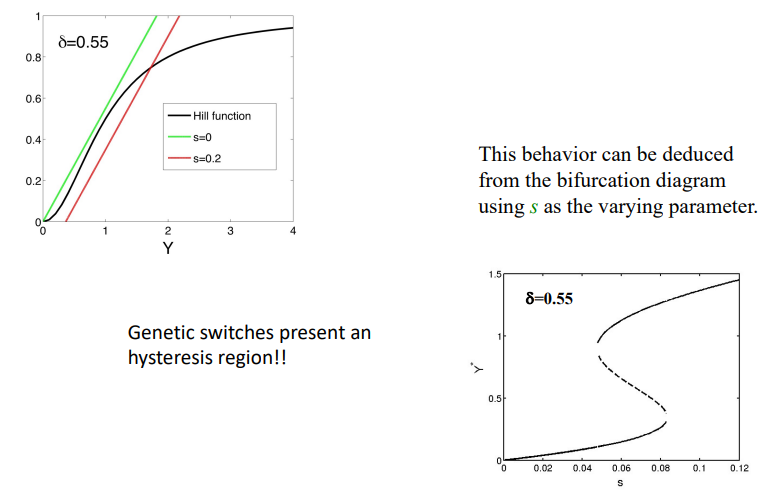
\includegraphics[width = \textwidth]{figs/genetic-switch.png}
\end{figure}

Si pintamos los puntos de equilibrio en valor del parámetro $s$, vemos que se produce una región de histéresis. 

Cuando hay interacciones mutuas con una variable y dos autorregulaciones positivas o negativas, hay más estados posibles: que se expresen los dos, ninguno o solo uno de ellos. En la activación mutua, si ambos son 0, no hay activación. Si con una señal se produce un poco de x, aumenta, activando y, llegando un momento en el que los dos pasan a estar expresados de forma máxima ($(0,0) \rightarrow (1,1)$). Si después se quita la señal, los estados siguen aumentados, no disminuyen debido a la histéresis. Un estímulo transitorio se convierte así en una respuesta permanente, a lo que se llama memoria celular. En una inhibición mutua, si un gen está expresado, el otro se reprime: $(0,1) \rightarrow (1,0)$
\begin{figure}[h]
\centering
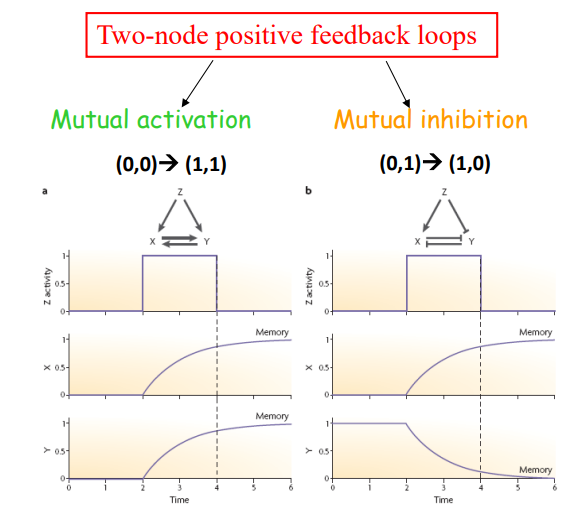
\includegraphics[width = 0.6\textwidth]{figs/cellular-memory.png}
\end{figure}

Si se combinan las retroalimentaciones positivas y negativas, se pueden dar los cuatro estados: $(0,0), (0,1), (1,0), (1,1)$. Esto se ha demostrado útil en la diferenciación de células madre.

\begin{figure}[h]
\centering
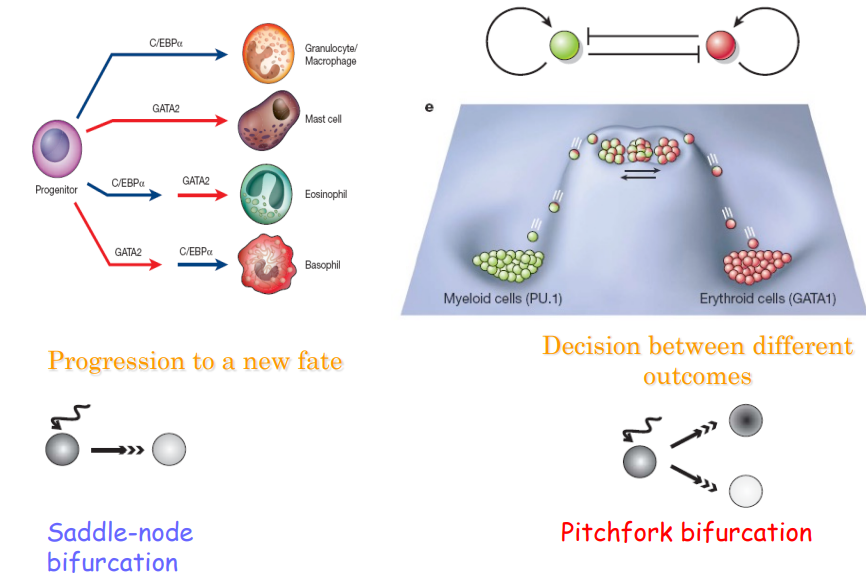
\includegraphics[width = 0.8\textwidth]{figs/stem-differentiation.png}
\end{figure}

Se puede representar un paisaje epigenético que describe los valles y colinas con los distintos destinos celulares. Las redes de regulación celulares dan lugar a que se enciendan o apaguen distintos genes en distintos estados. 

\begin{figure}[h]
\centering
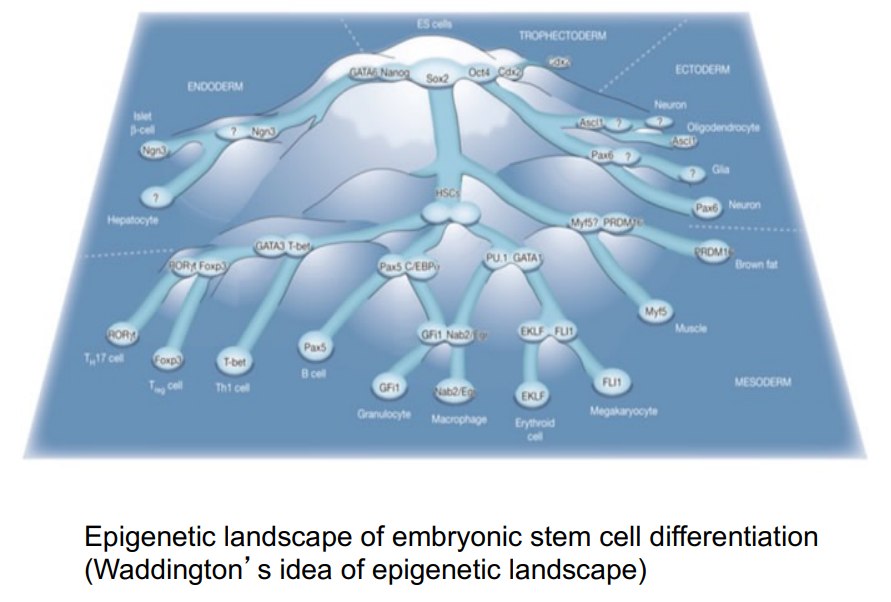
\includegraphics[width = 0.8\textwidth]{figs/waddington.png}
\end{figure}

\subsection{Feedback negativo y oscilaciones}
Hay muchos procesos fisiológicos y de señalización celular regulados por ritmos periódicos y oscilaciones. Los ritmos circadianos son comunes a muchos organismos, tanto mamíferos como bacterias o levaduras. La información está codificada en la frecuencia y el número de pulsos, como puede ser la activación de genes selectivos por factores de transcripción, señalización de calcio, respuesta a estrés, etc. En todos los ejemplos se han identificado proteínas o reguladores que interaccionan con las proteínas fundamentales de las respuestas mediante un feedback negativo. 

\begin{figure}[h]
\centering
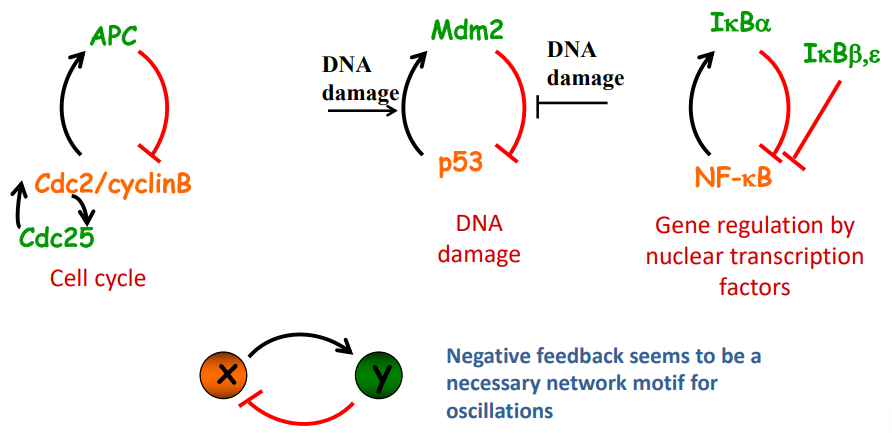
\includegraphics[width = 0.8\textwidth]{figs/feedback-negativo.png}
\end{figure}

Suponiendo que tenemos dos proteínas que interaccionan mediante un feedback negativo: una favorece a otra, la cual inhibe a la primera. Los mecanismos por los que un modelo dinámico oscila de forma robusta son los ciclos límite. Todos los ejemplos que tienen oscilaciones son debidos a los ciclos límite. Las condiciones para que haya un ciclo límite es la existencia de un punto inestable en el centro, el cual se denomina como espiral inestable. El tipo de bifurcación en el que una espiral estable pasa a inestable se conoce como bifurcación de Hopf, la cual implica la creación de un ciclo límite. Las espirales son autovalores complejos de la matriz jacobiana. Para un sistema de dos variables, hay una función $f(y)$ y una función $g(x)$, siendo la matriz jacobiana la matriz con las derivadas de las funciones en el punto de equilibrio. Los autovalores se pueden oner como la traza de las dos variables. Para tener bifurcación Hopf, el determinante debe ser positivo y la parte real debe pasar por 0, lo que equivale a que la traza pase por 0. 

Suponemos dos genes con interacciones mutuas. La producción de x depende de y. Suponemos que el término de degradación es $\delta x,y$.
$$\frac{dx}{dt} = f(y) - \delta x$$
$$\frac{dy}{dt} = g(x) - \delta y$$

La matriz jacobiana sería de la siguiente forma:
$$\vec{J} = \begin{pmatrix}
- \delta & \frac{\sigma f}{\sigma y} \\
\frac{\sigma g}{\sigma x} & - \delta
\end{pmatrix} \rightarrow \begin{pmatrix}
\text{Efecto de X sobre X} & \text{Efecto de Y sobre X} \\
\text{Efecto de X sobre Y} & \text{Efecto de Y sobre Y}
\end{pmatrix}$$
Así, la traza siempre va a ser negativa ($-2 \delta$). La matriz debe tener la siguiente estructura:
$$\vec{J} = \begin{pmatrix}
+ & + \\
- & -
\end{pmatrix}$$
o
$$\vec{J} = \begin{pmatrix}
+ & - \\
+ & -
\end{pmatrix}$$

Los elementos de las dos diagonales deben tener signos distintos para que pueda aparecer un ciclo límite. Para conseguir un signo positivo en la diagonal es mediante la autorregulación positiva de x o de y. El jacobiano representa el efecto de cada una de las variables sobre ellas mismas (en la diagonal) o sobre la otra (no diagonal).

\begin{figure}[h]
\centering
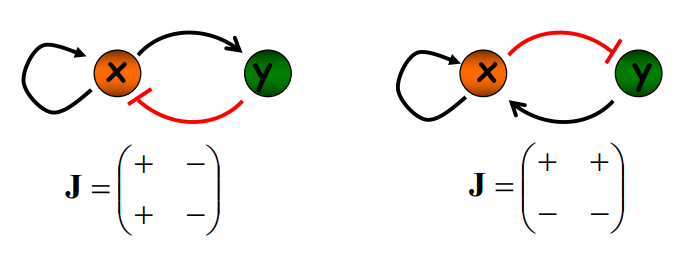
\includegraphics[width = 0.8\textwidth]{figs/feedback-jacobiano.png}
\end{figure}

Sin feedback negativo, no habría determinante positivo y, por tanto, ciclo límite. Se necesita feedback negativo, pero con autorregulación positiva. El signo positivo de la diagonal implica una autorregulación positiva, mientras que el signo negativo no implica autorregulación negativa, si no que hay degradación y no hay autorregulación. 

Por lo tanto, para que existan oscilaciones en redes de dos componentes, en principio son necesarias tanto la retroalimentación negativa como la autorregulación positiva (un ejemplo es el oscilador del ciclo celular). En el caso del modelo Lotka-Volterra, la autorregulación positiva sería la tasa de crecimiento por reproducción, mientras que la retroalimentación negativa es la interacción presa-predador. 

El feedback positivo no es estrictamente necesario, ya que el feedback negativo produce un desfase temporal entre las interacciones que ya produce las oscilaciones. El motivo de retroalimentación negativa más simple, la autorregulación negativa, puede mostrar oscilaciones si se introduce explícitamente un retraso en la transcripción y traducción del gen.

El retraso en el módulo combinado de retroalimentación negativa con autorregulación positiva viene dado por el bucle de retroalimentación positiva que ralentiza las respuestas.

\begin{figure}[h]
\centering
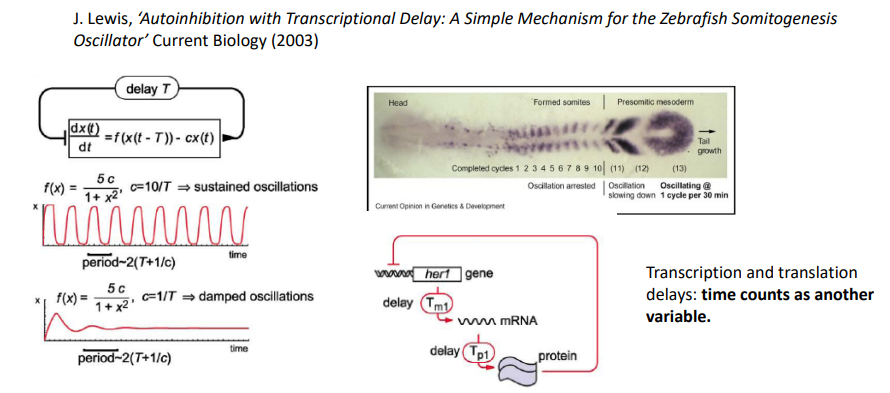
\includegraphics[width = 0.8\textwidth]{figs/autoinhibition-delay.png}
\end{figure}

Los osciladores con retroalimentaciones negativas y positivas entrelazadas aparecen con más frecuencia en los sistemas biológicos debido al principio de robustez: El periodo y la amplitud de las oscilaciones no deben variar tanto con el ruido molecular. El oscilador con retroalimentación positiva es mucho más robusto frente a las fluctuaciones naturales en la abundancia de los componentes. 

\end{document}
